\documentclass[tikz]{standalone}

\begin{document}
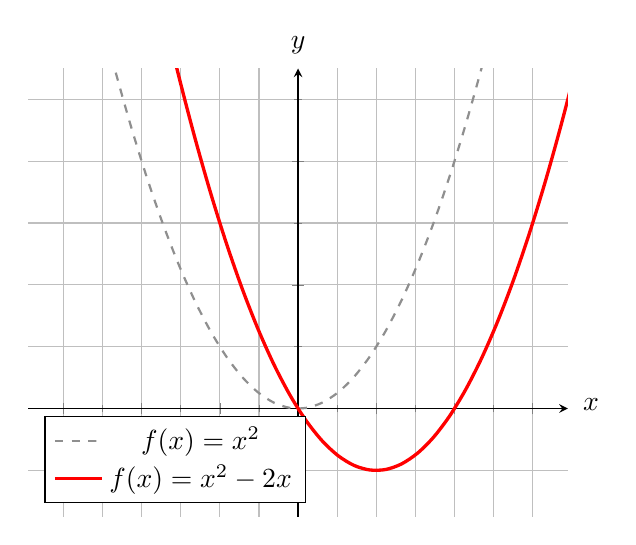
\begin{tikzpicture}
    \begin{axis}[%
        xlabel=$x$, ylabel=$y$, legend pos=south west,
        grid=both, xmin=-3.45, xmax=3.45, ymin=-1.75, ymax=5.5,
        axis lines = middle,
        minor x tick num=1, minor y tick num=1,
        xlabel style = {at={(axis description cs:1.01,0.25)},anchor=west},
        ylabel style = {at={(axis description cs:0.5,1.01)},anchor=south},
        xticklabels = {}, yticklabels={},
    ]
    \addplot[lightgray!75!black, thick, dashed, domain=-5:5, smooth, samples=50] plot {x^2};
    \addplot[red, very thick, domain=-5:5, smooth, samples=50] plot {x^2-2*x};
    \legend{$f(x)=x^2$,$f(x)=x^2-2x$}
    \end{axis}
\end{tikzpicture}
\end{document}
